

\chapter{Readout Infidelity Budget} \label{chap:readout_infidelity_budget}
With a simulation realistically representing the qubit-resonator system from the laboratory, we are now in a position to break down the different effects on the readout fidelity. In this section, we will leverage the simulation tools, to quantify the contributions to the infidelity from the different physical processes, we have included in our model. Thereafter, we will try to break down, how different improvements of the physical parameters will have an effect on the fidelity of our readout. 

\section{Turning off the Contributions}
From the different calibration in chapter \ref{sec:calibrations} and the readout analysis in section \ref{sec:readout}, we hypothesize three main contributions to our readout (and initialization error):
\begin{enumerate}
    \item The measurement efficiency, $\eta$. To get two non-overlappping measurements, we need to limit the noise is added to the states of the resonator. 
    \item The temperature, $\tau$, is contributing significantly to the initialization error. At non-zero temperature, we will expect to see a mixed state with non-zero elements for $\ket{1}\bra{1}$ and $\ket{2}\bra{2}$. 
    \item Characteristic time for energy decays, $T_1$. Since relaxation or excitation during the readout will make the system behave like it is in the other state, this will lead to wrong classifications.
\end{enumerate}


\begin{figure}
    \centering
    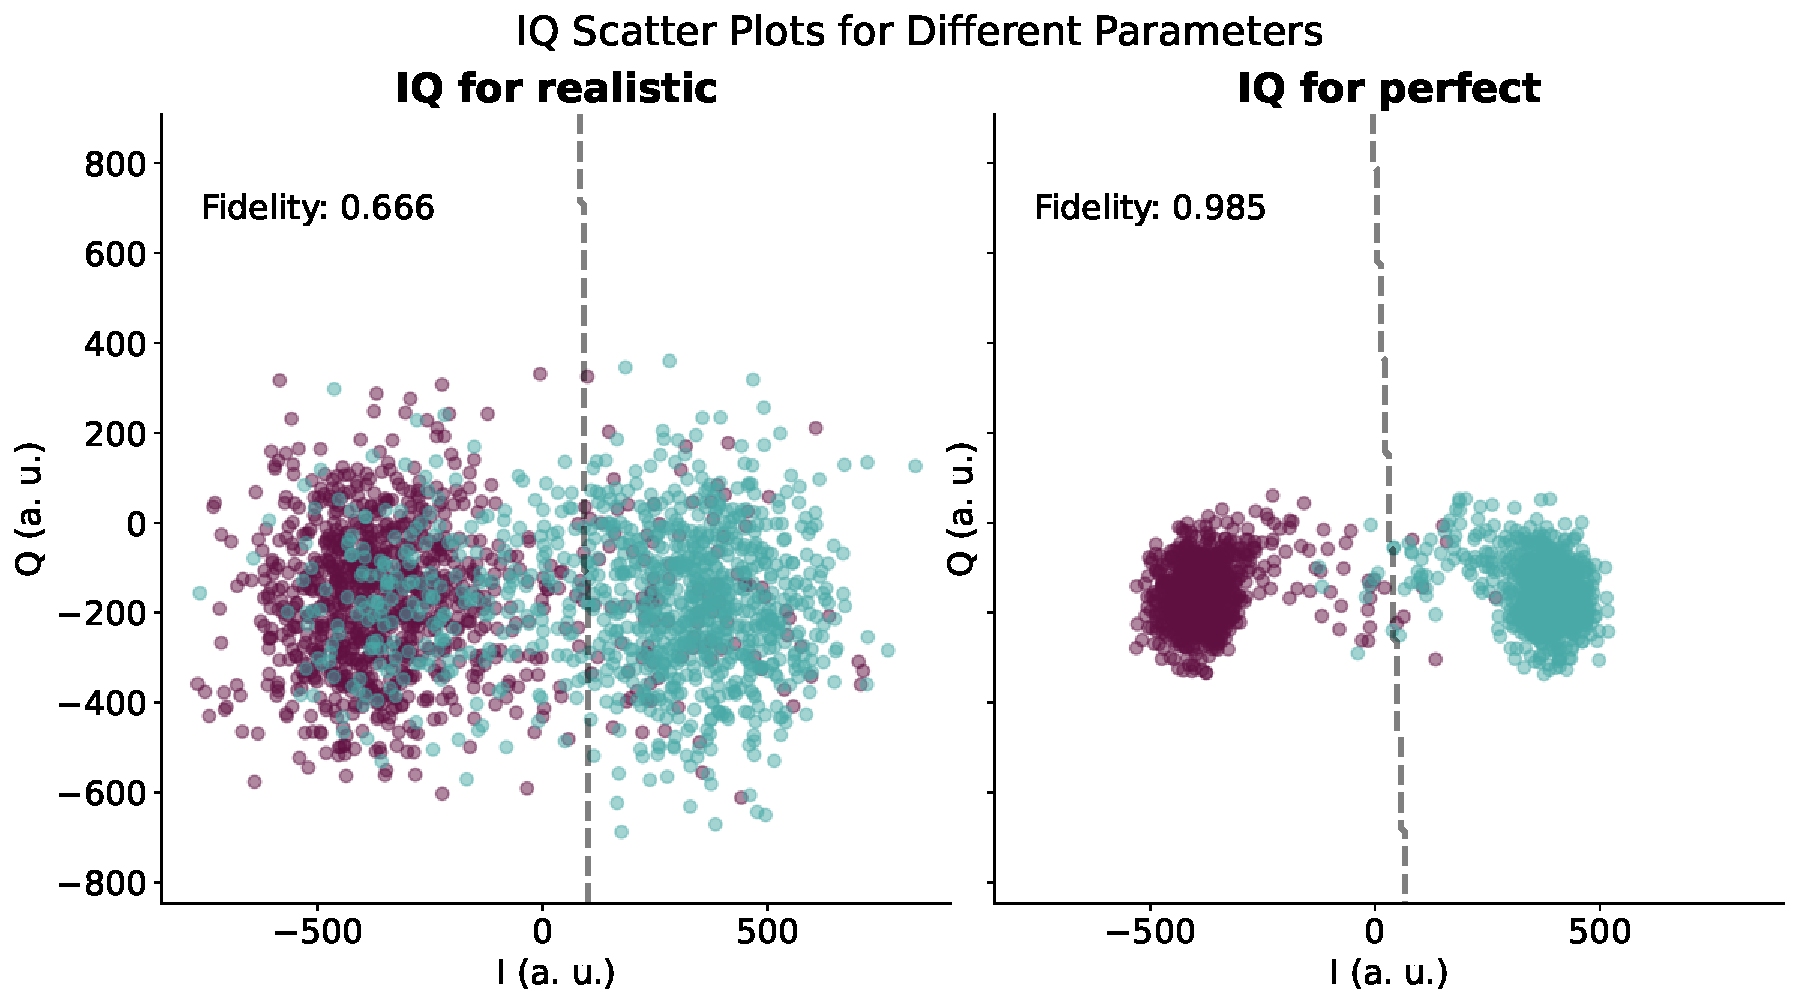
\includegraphics[]{Simulations/budgets/figures/iq_scatter_budgetting_on_off_two.pdf}
    % \missingfigure[figheight = \textheight / 3]{IQ Plots for the simulation, we ran in the table}
    \caption{The IQ distributions for the experiment run with a realistic and an ideal set of parameters. The fidelity as well as separation line is shown on the plot. }
    \label{fig:realistic_perfect_comparison}
\end{figure}

\begin{margintable}
    \centering
    \caption{Results from running the simulation experiment for a thousand samples with a realistic set of parameters and a perfect set of parameters. The uncertainities are calculated by assuming binomial distribution with the false positive and negative rate and dividing by the amount of samples. $\sigma = \sqrt{p (1-p) / N}$ and the adding them in quadrature to the standard error on $1 - \text{fpr} - \text{fnr}$}
    \begin{tabular}{l|r}
    \hline
         Parameters Set & Fidelity \\ \hline
         Realistic & 0.666 $\pm$ 0.012  \\
         Perfect   & 0.985 $\pm$ 0.003
    \end{tabular}
    \label{tab:realistic_perfect_comparison}
\end{margintable}

By using the model which we built up in chapter \ref{sec:building_simulation}, we can now turn off the different contributions to see the outcome. As a start, we see what happens, if we happened to have a qubit with infinite lifetime $T_1 = \infty$, a fridge capable of bringing the qubit to zero temperature $\tau = 0$ and an amplification chain which do not lose any information in the readout process $\eta = 1$. A comparison of the Fidelity of this perfect system and the realistic one, which we also simulated in section \ref{sec:readout_in_simulation} can be seen in table \ref{tab:realistic_perfect_comparison} and the corresponding IQ plot is found in figure \ref{fig:realistic_perfect_comparison}. \textbf{To see the weights and histrograms for calculating these plots as well as the following IQ plots, refer to appendix \ref{appendix}}.



\textbf{Comment on the actual results here. Something like} Notice that with perfect parameters the IQ plot shows two very well defined and pure plots far away from each other \textbf{without} tails leading from on the other. This is further supported by a readout fidelity of $... $. 




In an attempt to single out the effect on readout fidelity from the individual contributions, we can repeat the experiment with the different combinations of turning the effects on one after another. This leads to six experiments. Starting from the realistic set of parameters, we have three experiments with $\eta = 1$, $T_1 = \infty$, $\tau = 0$ respectively (excluding a source of SPAM error). And then three examples where any two of the above is applied (such that the error is exclusively from one parameter according to the hypothesis). The IQ plots can be seen in figure \ref{fig:on_off_IQ_scatter_combinations} and the associated fidelity scores in table \ref{tab:readout_infidelity_contribution_estimation}.

\begin{figure}[h]
    \centering
    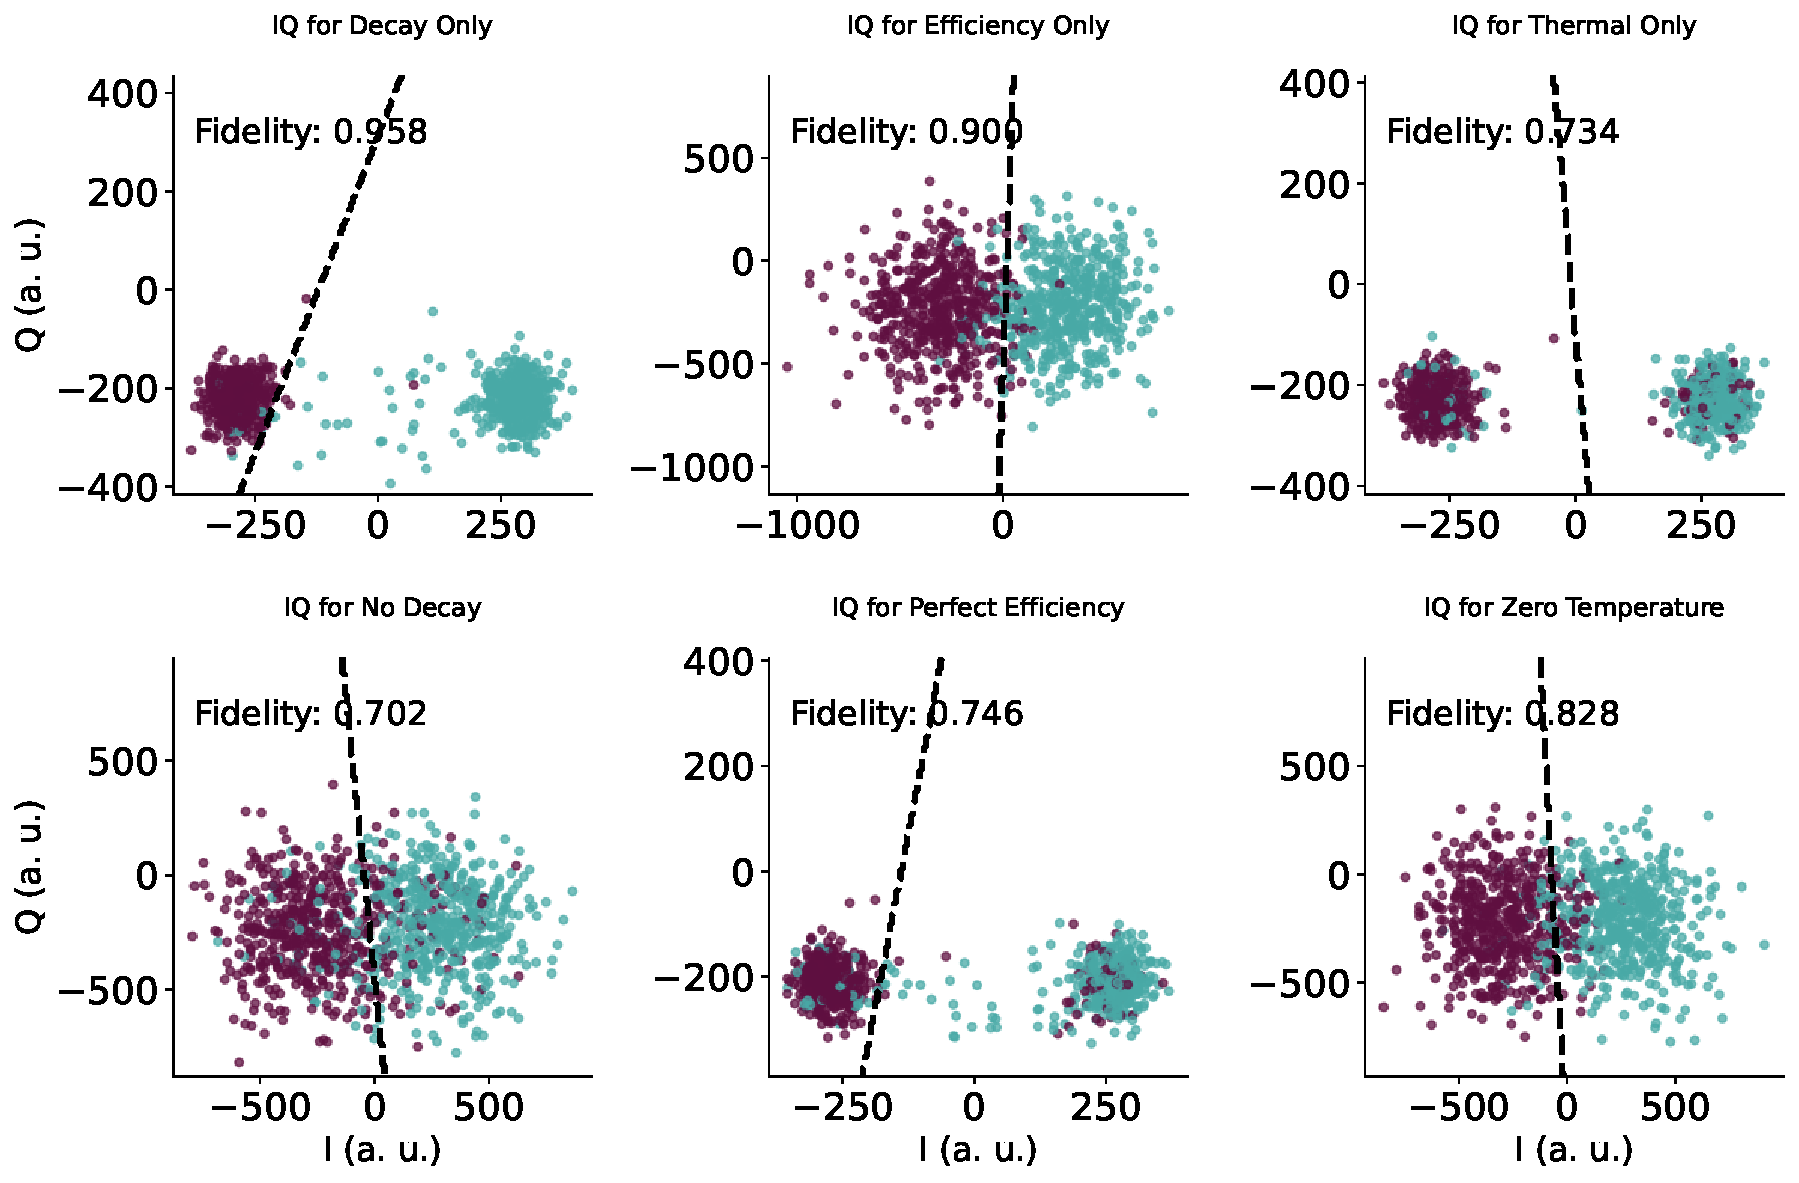
\includegraphics[]{Simulations/budgets/figures/iq_scatter_budgetting_on_off.pdf}
    % \missingfigure[figheight = \textheight / 3]{IQ Plots for the simulation, we ran in the table}
    \caption{The IQ results from turning on the different sources of errors one by one. The IQ scatter plots are displayed along side the decision boundary and the readout fidelity.}
    \label{fig:on_off_IQ_scatter_combinations}
\end{figure}

\begin{table}[h]
\centering
\caption{The Fidelity results of running the simulation experiment with 1000 samples given parameters that sets one or two of the three parameters to the ideal setting.}
\begin{tabular}{l|rrr}
\hline
\textbf{Contributions}        & Temperature         & Energy Decay   & Efficiency  \\ \hline
Excluding                     &  0.878 $\pm$ 0.008  &  0.710 $\pm$  0.011  &  0.655 $\pm$ 0.012\\
Exclusively                   &  0.721 $\pm$ 0.011  &  0.879 $\pm$  0.008  &  0.982 $\pm$ 0.003
\end{tabular}
\label{tab:readout_infidelity_contribution_estimation}
\end{table}



\begin{figure*}
    \centering
    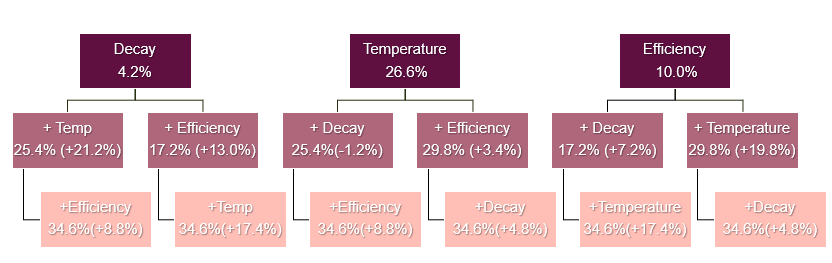
\includegraphics{Figs/Results/combination_tree.png}
    \caption{Visualizing the different ways of combining the error sources and watching their contributions at each step.}
    \label{fig:combination_tree_budget}
\end{figure*}


Another way of visualizing these parameters are by having them in a combination tree and combining them in different ways. Each time we add a new source of errors we can find the increase in infidelity. This will allow us to get a good idea of the contribution from the individual sources. This is done in figure \ref{fig:combination_tree_budget}. We see clearly that the effects are not separable and the contribution of a parameter is different depending on which error sources are present. However, to get vague estimate, we can take the average over infidelity contributions for the different parameters. These averages are shown in table \ref{tab:average_combination_tree}. 
\begin{margintable}
    \centering
    \begin{tabular}{l|r}
    \hline
    Parameter       &  Avg Infidelity\\ \hline
    Temperature     & 0.221 ? \\
    Decay           & 0.098 ? \\
    Efficiency      & 0.015 ? \\
    \end{tabular}
    \caption{Average contribution to infidelity when counting in the combination tree seen in figure \ref{fig:combination_tree_budget}}
    \label{tab:average_combination_tree}
\end{margintable}

\textbf{For the system considered in this thesis, it can be see that the biggest contributions to the uncertanity is... }





\section{Improving the Readout}
In the previous section, we gave some estimates on how much three different sources contributed to the infidelity in the readout and initialization process. Although these numbers are interesting, an ideal qubit with infinite lifetime or a cooling system capable off sub mini kelvin temperatures are not realistic and is probably not what one should strive for. Instead, we will in this section present more marginal improvements like what would happen if the temperature is reduced by 10\% or 25\%. Furthermore, we will cover some strategies which can be implemented to deal with some of the errors in the straightforward 1 µs readout pulse which we have considered until now.

\subsection{Modifying the Parameters}
\begin{figure*}[t]
    \centering
    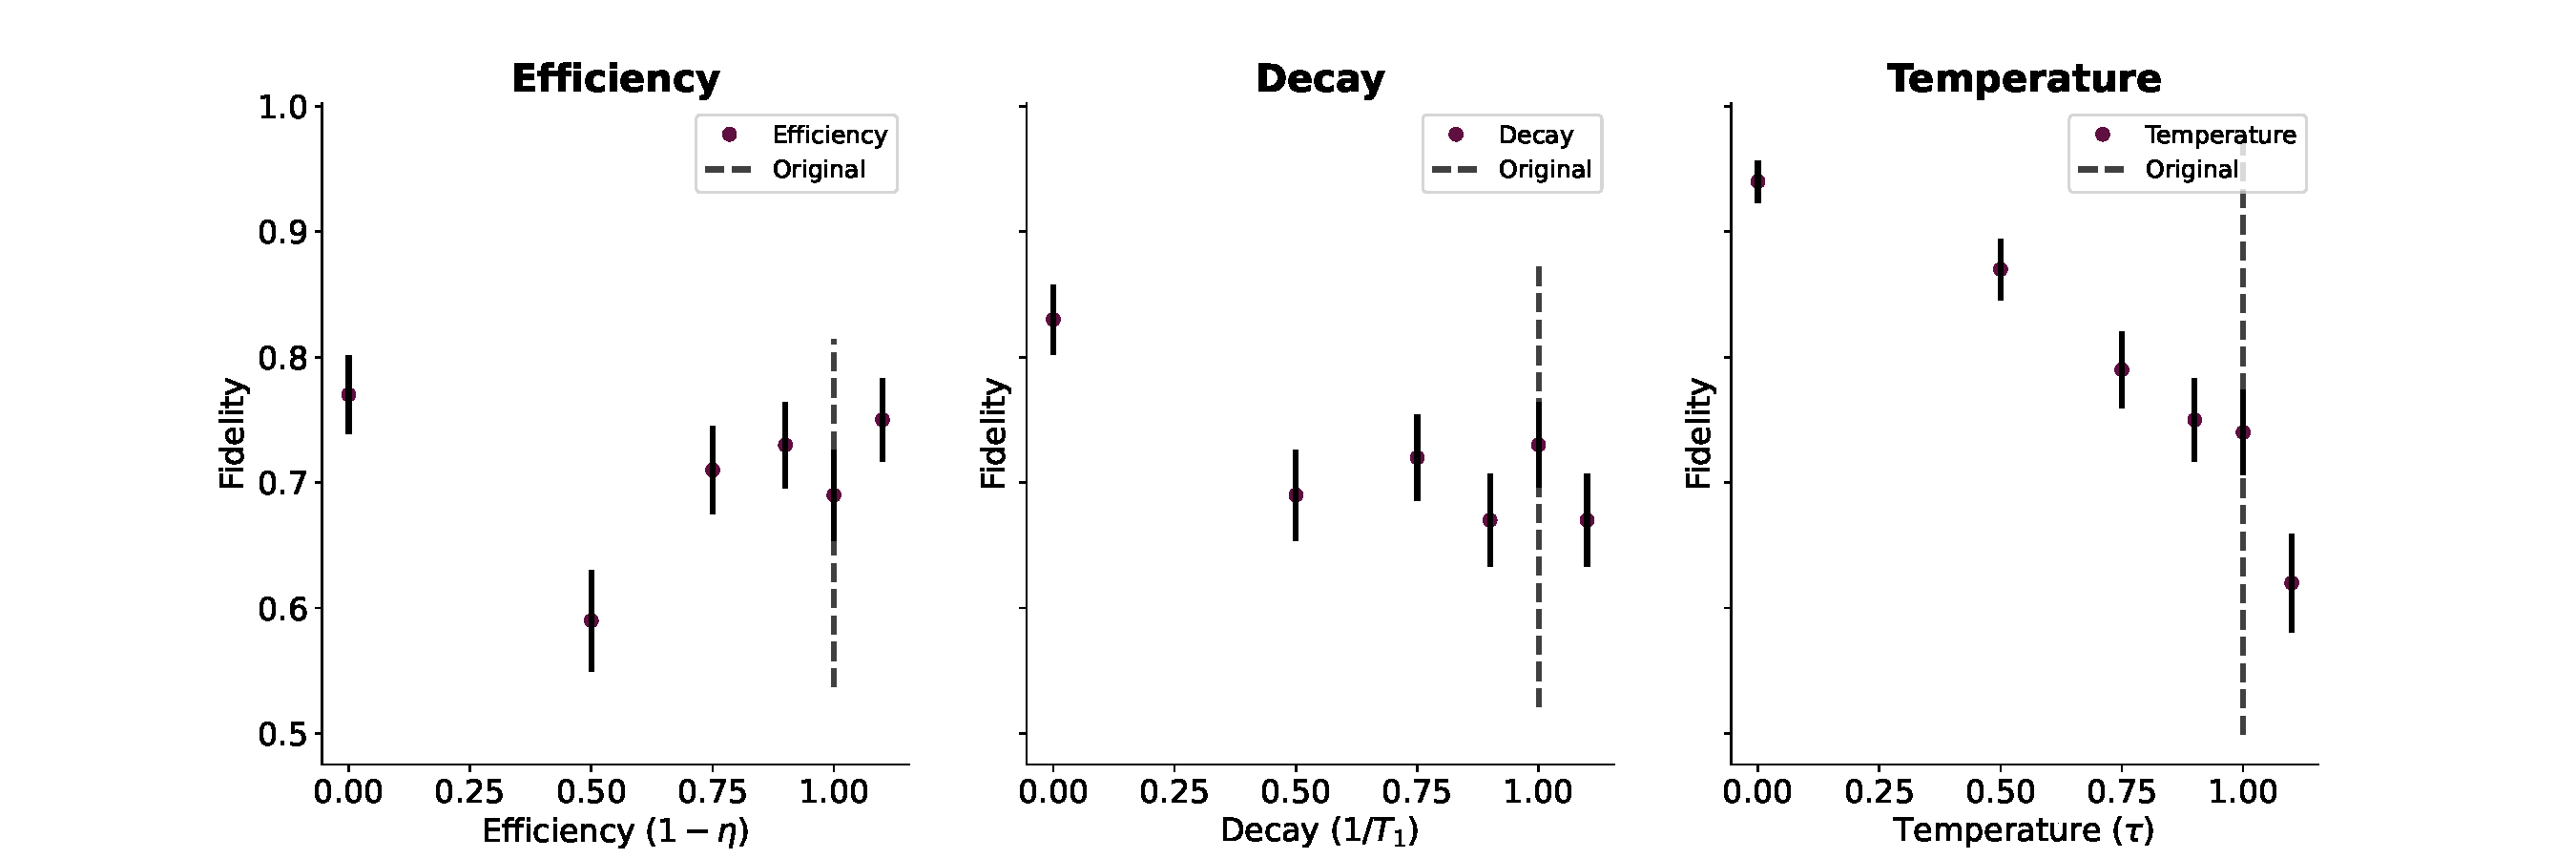
\includegraphics[width = \linewidth]{Simulations/budgets/figures/fidelities_at_different_parameters.pdf}
    \caption{The Fidelities of the model when the parameters are changed. In each plot the two other parameters are held constant at the realistic value.}
    \label{fig:scan_of_fidelities_at_different_parameters}
\end{figure*}
In the previous section, we considered the parameters to be $0$ or $100 \%$ of the considered value. In this section, we will instead create experiment with fractional improvements compared to the system parameters. To make the comparison somewhat fair, we will make sure to define quantities such that $0\%$ is perfect thus we will try different values for decay rate $\Gamma_1 = 1 / T_1$, inefficiency $1 - \eta$ and temeprature $\tau$. For each of these parameters, we run an experiment with the value at $0, 50\%, 75\%, 90\%, 100\%$ and $110\%$ of the initial value while keeping the other two parameters fixed. The results can be seen in figure \ref{fig:scan_of_fidelities_at_different_parameters} and in the tables: \ref{tab:temperature_contribution_estimation}, \ref{tab:decay_contribution_estimation} and \ref{tab:readout_infidelity_contribution_estimation}. The IQ plots of for the different experiments can be seen in, \ref{fig:budgetting_IQ_plots} and to see the weights and histogram used to calculate the fidelity refer to appendix \ref{appendix}... 


\subsection{Temperature}
In our model, the temperature has two roles: to determine the mixed state in the beginning of the readout and the relation between energy excitation and decays. Especially, the first of these two affects increases the SPAM error significantly as it can not be distinguished in the readout process. In table \ref{tab:temperature_contribution_estimation}, we can also see the increase in fidelity from decreasing the temperature. 


\begin{table}[h]
\centering
\caption{The outcome of calibrating the qubit with the methods presented in this chapter for different temperatures.}
\begin{tabular}{ll|r}
\hline
\textbf{Reduction}        & Temperature                  & Fidelity\\ \hline
-10 \%                     &  30                         &  99.99\\
0   \%                     &  30                         &  99.99\\
10  \%                     &  30                         &  99.99\\
25  \%                     &  30                         &  99.99\\
50  \%                     &  30                         &  99.99\\
100 \%                     &  30                         &  99.99\\
\end{tabular}
\label{tab:temperature_contribution_estimation}
\end{table}

\textbf{Do I have anything else to say here???} 


\paragraph{Active Reset - } One way of artificially "cooling down" the qubit is by initializing by readout. If the readout fidelity is larger than the state preparation, we will now have a mixed state of $\rho = .... $ if we measure $\ket{0}$ and if you measure $\ket{1}$, we can apply an X-gate to return to the above\footnote{Up to a gate fidelity which however is a few order of magnitude lower than the other errors considered in this thesis and thus neglected}. 

To gain an advantage from active reset, we require the qubit to have long coherence time and high efficiency. The long coherence time is necessary since a normal readout tries to determine the state at the beginning of the pulse, but since an x-gate should only be performed if the qubit is in state $\ket{1}$ at the end of the pulse it should not decay in the meantime. In addition, to make sure we can neglect the gate fidelity of the X-gate, we need to wait (or do a counter pulse on the resonator \cite{}) to empty it for photon otherwise the qubit frequency will be shifted by the photons in the resonator and the qubit will be initialized poorly and the first few gates of a desired circuit will also be off. 

\subsection{Qubit Decay}
Unwanted changes of the qubit between $\ket{0}\leftrightarrow\ket{1}$ is also a big barrier to reading out the qubit. Since the qubit can change state during the readout process, it will be difficult to classify as either $\ket{0}$ or $\ket{1}$. Since it will often create tails going from one to the other. In table \ref{tab:decay_contribution_estimation}, we see how small reductions in the transition rate increase the readout fidelity. 

\begin{table}[h]
\centering
\caption{The outcome of calibrating the qubit with the methods presented in this chapter.}
\begin{tabular}{lll|r}
\hline
\textbf{Reduction}         &  $\Gamma_1$                  &  $T_1$                & Fidelity\\ \hline
-10 \%                     &  30 $\text{µs}^{-1}$         &  3.00 µs             &  99.99\\
0   \%                     &  30 $\text{µs}^{-1}$         &  3.00 µs             &  99.99\\
10  \%                     &  30 $\text{µs}^{-1}$         &  3.00 µs             &  99.99\\
25  \%                     &  30 $\text{µs}^{-1}$         &  3.00 µs             &  99.99\\
50  \%                     &  30 $\text{µs}^{-1}$         &  3.00 µs             &  99.99\\
100 \%                     &  30 $\text{µs}^{-1}$         &  3.00 µs             &  99.99\\
\end{tabular}
\label{tab:decay_contribution_estimation}
\end{table}

In section \ref{sec:post_selection}, we saw that we can remove most of the $T_1$ decay by increasing an overhead, however this will severely impact the ability to run codes and will not be feasible in scenarios like error correcting codes, where a readout is performed on 10s or 100s of qubit in every cycle.   \todo{Can we show this in simulation as well, if we do postselection for all of the $T_1$ experiments}

\paragraph{Shorter Readout Pulse - } One way of decreasing the effect of $T_1$ on readout fidelity is clearly by making a shorter readout sequence. This will require a greater efficiency since the standard deviation of the ground and excited distributions in the IQ space scales with $1 / \sqrt{\eta t_{\text{readout}}}$. So to assure that the distributions are at least 2-3 standard deviations apart to get sub-percent overlap, this sets a requirement for the fidelity.

\paragraph{Further Excitement - } Another method for reducing the impact is by applying a gate pulse at $f_{12}$ such that $\ket{1}\to\ket{2}$ while $\ket{0}$ stays in $\ket{0}$. Now the readout frequency can be altered to make sure that the Q-function for $\ket{1}$ and $\ket{2}$ are close and easily separable from $\ket{0}$. Since the second excited state $\ket{2}$ first will have to decay to $\ket{1}$ before decaying to $\ket{0}$ \todo{Footnote about fermis golden rule and how this supresses the direct transition} it will increase the readout fidelity. This however comes at the cost of not classifying $\ket{0}$ or $\ket{1}$, but will instead give us $\ket{0}$ or $\ket{\text{not }0}$ since the state could have been in either of the excited states in the measurement. For this reason the further excitement can not be combined with the active reset method presented in the previous subsection.

\subsection{Efficiency}
The efficiency plays a delicate role for reading out. Since we to a rough estimate get two Gaussian distributions in the IQ plot in the readout process, the overlap scales with the amount of standard deviations they are apart. While having a distance at $< 3\sigma$ give an overlap of order a few percent, this drops rapidly after and when the distributions are $5 \sigma$ apart the overlap is negligible especially compared to the contributions from decay and temperature. To see the effect of reducing the inefficiency refer to table \ref{tab:readout_infidelity_contribution_estimation}. 

\begin{table}[h]
\centering
\caption{The outcome of calibrating the qubit with the methods presented in this chapter.}
\begin{tabular}{lll|r}
\hline
\textbf{Reduction}        & Inefficiency    & Efficiency                    & Fidelity\\ \hline
-10 \%                    &  30 \%          &  30 \%                        &  99.99\\
0   \%                    &  30 \%          &  30 \%                        &  99.99\\
10  \%                    &  30 \%          &  30 \%                        &  99.99\\
25  \%                    &  30 \%          &  30 \%                        &  99.99\\
50  \%                    &  30 \%          &  30 \%                        &  99.99\\
100 \%                    &  30 \%          &  30 \%                        &  99.99\\
\end{tabular}
\label{tab:readout_infidelity_contribution_estimation}
\end{table}

In the table we see .... 

\paragraph{High Power Readout - } The efficiency helps reduce the overlap of the two distribution by making the distributions narrower. However, another approach is to move them further away from each other. In this thesis, we have been limited by the amount of photon number for numerical reason, but driving driving the resonator with a larger amplitude, the two distributions move further away in the IQ-space. One should however be aware of the increased shift of the qubit frequency and to still be within the critical photon number where the dispersive approximation is valid.

\begin{figure}
    \centering
    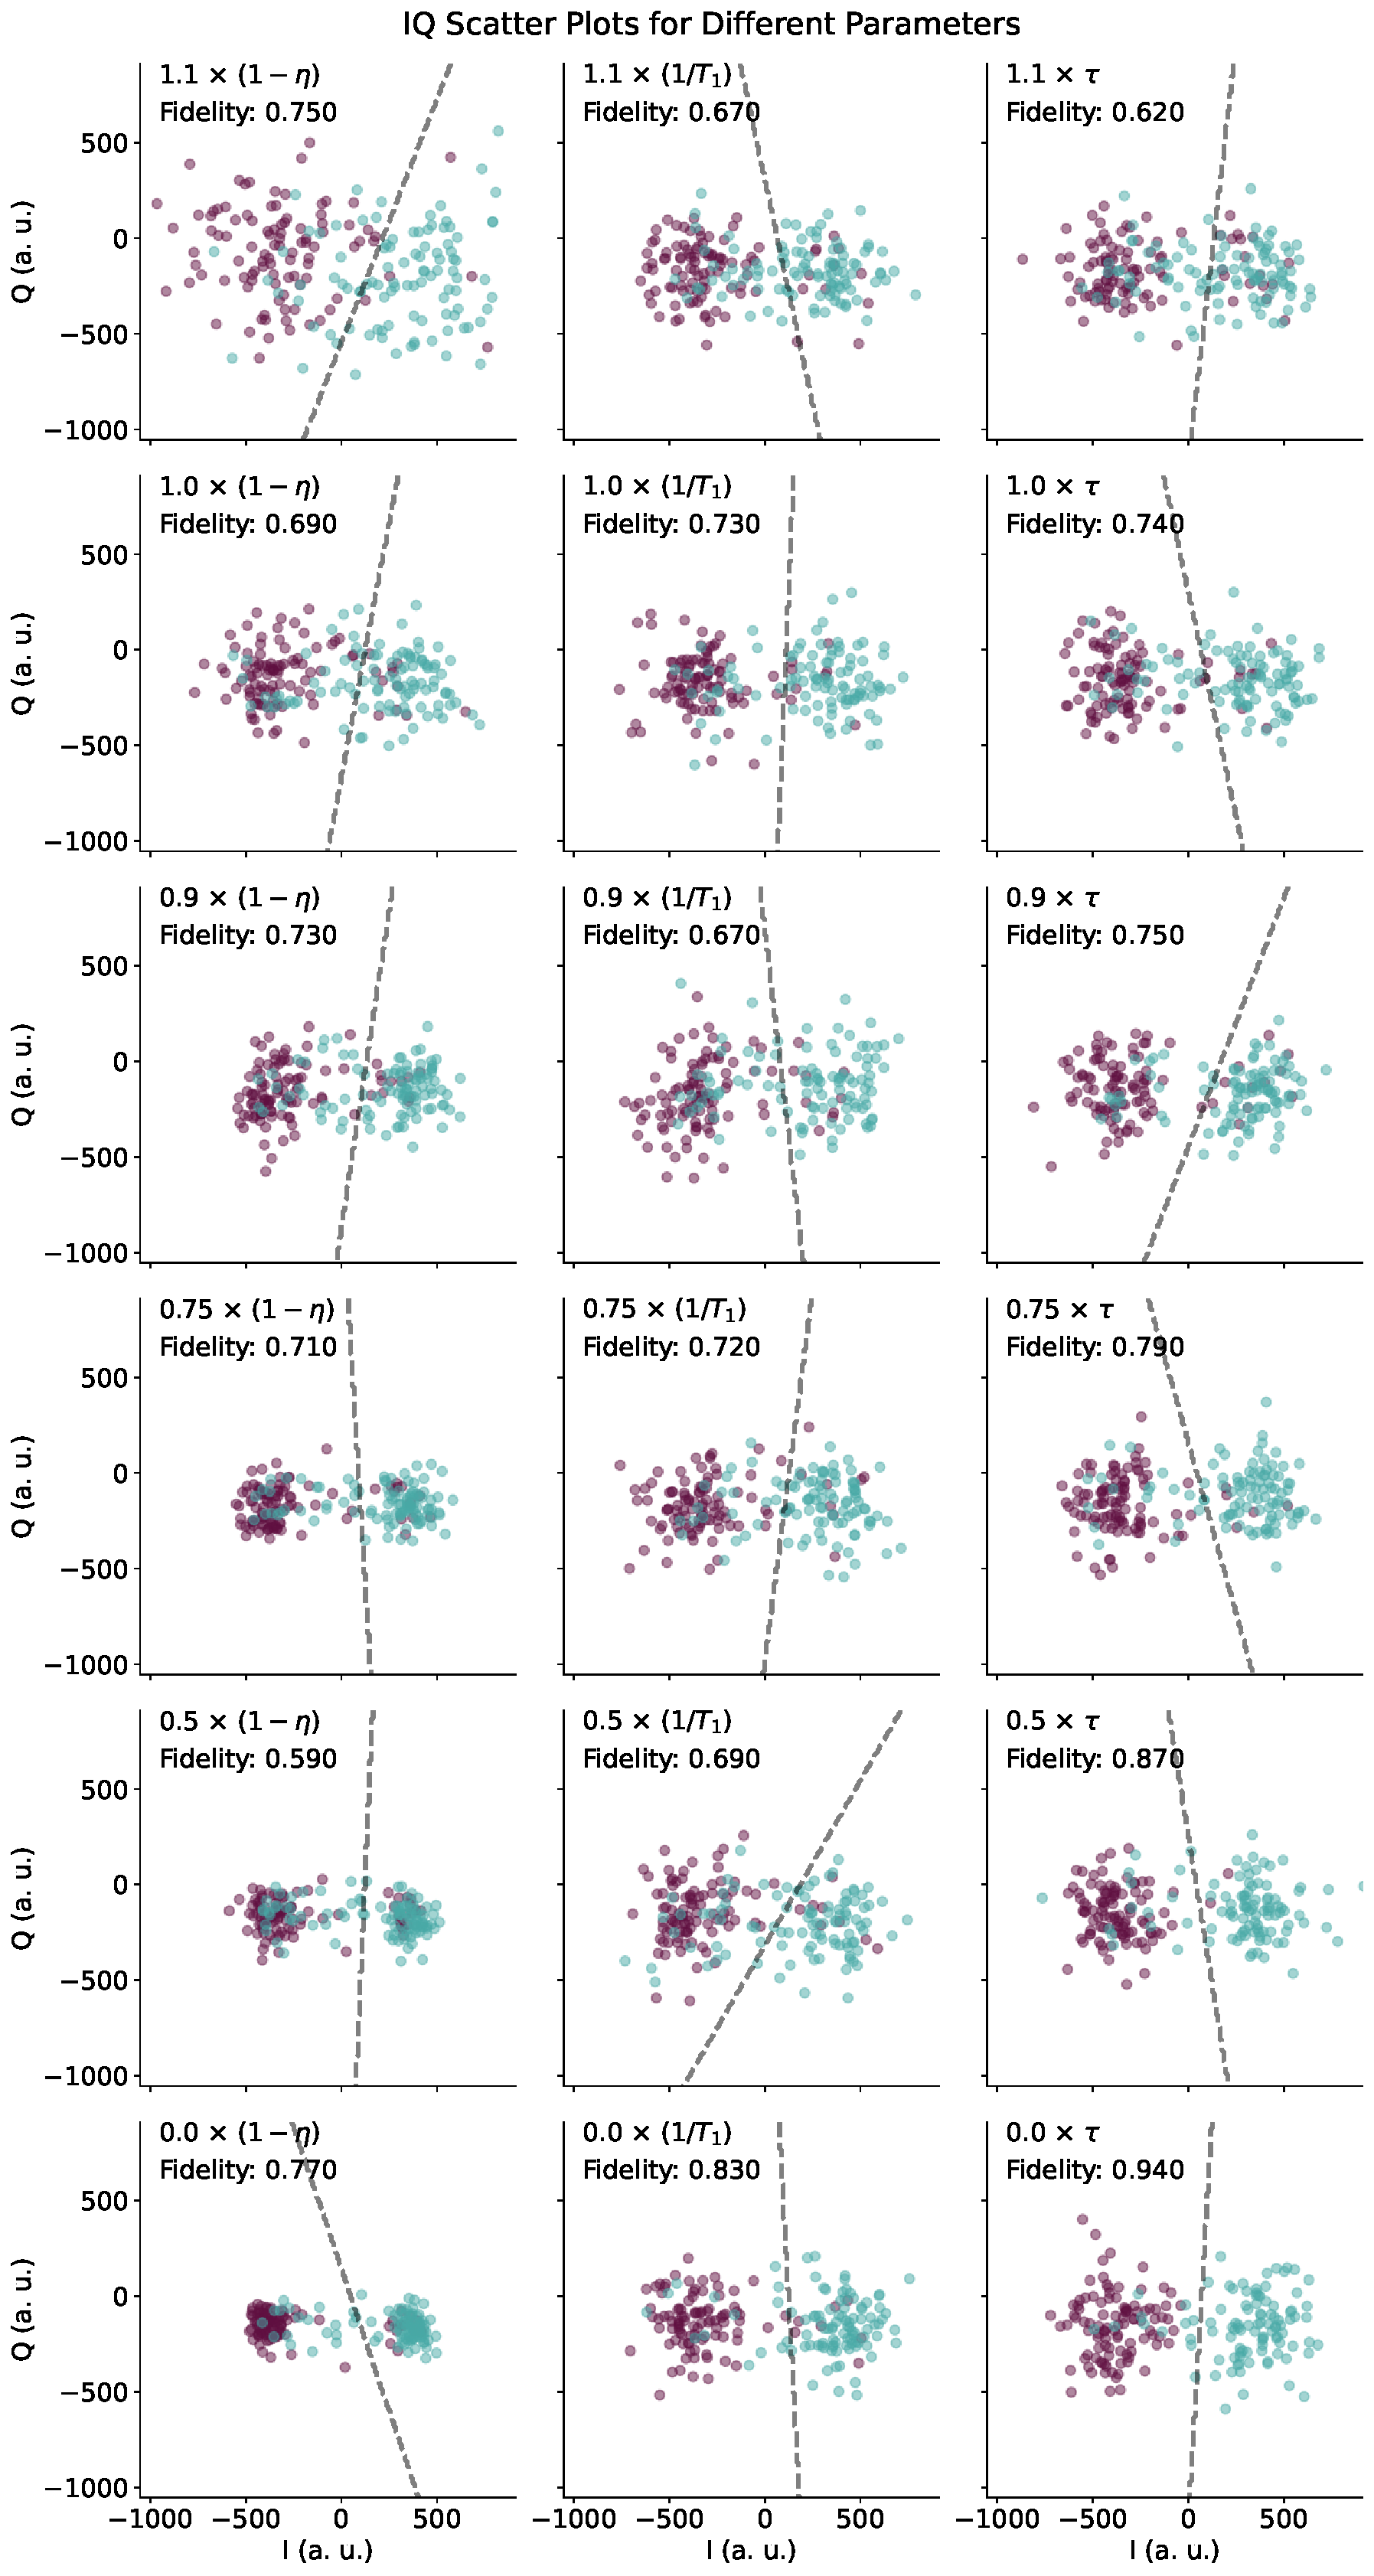
\includegraphics{Simulations/budgets/figures/iq_scatter_budgetting.pdf}
    \caption{The IQ Plots for the models  with different parameters. The seperation line, fidelity and parameter scaling is shown.}
    \label{fig:budgetting_IQ_plots}
\end{figure}

\FloatBarrier

\section{Further Path to Optimization}
In the sections above, we have very much considered a first order optimization, where all except one parameter was kept constant. This gives significant improvements for reductions in \textbf{temperature}, a bit less for increased $T_1$ and almost nothing for increasing the \textbf{efficiency}. In addition to the improvements from a colder, more coherent and more efficient setup, we also discussed the possibility of "trading" a good performing parameter to improvements in the others. Some of the trade-offs are illustrated in figure \ref{fig:trading_performance}. 

\begin{marginfigure}[- 2 cm]
    \centering
    \missingfigure{Trading parameters}
    \caption{Illustration of trading the good parameters to improvements in the others. }
    \label{fig:trading_performance}
\end{marginfigure}

\textbf{This is only right because, we increased the efficiency quiet a lot.}
For our system, we see that the contribution from efficiency is small. This is a result of the separation in even with the realistic parameter setting is of a few standard deviations, so the overlap is of order 1 \%, when we compare with $T_1$-decay and temperature, this is a very small contribution. Thus, we should prioritize a shorter pulse. Event though the overlap of the distributions will increase, the result will be less time for decay and should improve the overall fidelity. The same consideration can be made for $T_1$ which contributes less than the temperature. For this reason, active reset will result in a significant performance gain. 

The improvement gained by reducing the parameters in the section above are thus not very representative since we should start by changing the parameters to find the optimal readout duration, amplitude and applying some of the tricks (like active reset) if they increase the performance. In the case with the model built in this thesis, we should definitely decrease the pulse duration, turn up the amplitude and derive a way to simulate the process of doing active reset of the qubit. 

Even though the reduced readout duration is good news for the simulation process, the two others are definitely not. As discussed in section \ref{where} increasing the amplitude will force us to increase the dimensions of the Hilbert space as well. And since the Lindblad Equation and the Stochastic Master Equation both evolve the density matrix, we would effectively get $n^2$ differential equation to solve. Implementing active reset in simulation is also not trivial. In the code-module built for this thesis, the simulation of a trajectory is separate from the analysis and classification from the trajectories. In active reset, we would have to do a simulation, readout analysis and either apply an x-gate or not before simulating again\footnote{And might even have to repeat multiple times if the readout the second time still gives $\ket{1}$}. Since we also need to take into account the cool down of the resonator and the possibility of qubit decay in the meantime, this would ultimately mean a 3-10 times increase  (at best)  of simulation time and would require a much more flexible simulation module.